\subsection{中心对称、中心对称图形}\label{subsec:czjh1-4-8}

在前一章,我们学过关于直线对称的图形。
在日常生活和工农业生产中,还会遇到关于点对称的图形,
例如,飞机的螺旋桨,风车的风轮等,就是关于一点对称的图形的实例(图 \ref{fig:czjh1-4-29})。
它们的每个叶片转动 $180^\circ$ 后,都转到与它相对的叶片的位置。

\begin{figure}[htbp]
    \centering
    \begin{minipage}[b]{7cm}
        \centering
        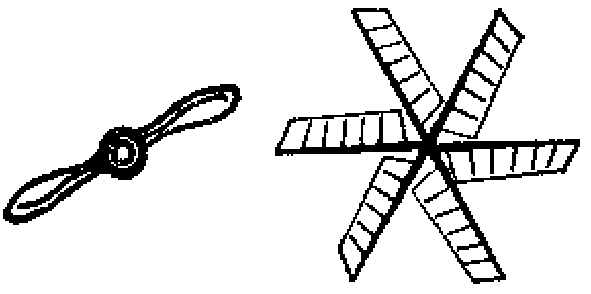
\includegraphics[width=6cm]{../pic/czjh1-ch4-29.png}
        \caption{}\label{fig:czjh1-4-29}
    \end{minipage}
    \qquad
    \begin{minipage}[b]{7cm}
        \centering
        \begin{tikzpicture}
    \tkzDefPoints{0/0/O,  1.1/-0.7/A,  1.8/0/B, 0.8/0.7/C}
    \tkzDefPointBy[symmetry=center O](A)  \tkzGetPoint{A'}
    \tkzDefPointBy[symmetry=center O](B)  \tkzGetPoint{B'}
    \tkzDefPointBy[symmetry=center O](C)  \tkzGetPoint{C'}
    \tkzDrawPolygon(A,B,C)
    \tkzDrawPolygon(A',B',C')
    \tkzDrawSegments[dashed](A,A'  B,B'  C,C')
    \tkzDrawArc[towards,dashed](O,A)(A')
    \tkzDrawArc[towards,dashed,red](O,B)(B')
    \tkzDrawArc[towards,dashed,red](O,C)(C')
    \tkzLabelPoints[below](A,C')
    \tkzLabelPoints[above](A')
    \tkzLabelPoints[above](O)
    \tkzLabelPoints[right](B)
    \tkzLabelPoints[left](C,B')
\end{tikzpicture}


        \caption{}\label{fig:czjh1-4-30}
    \end{minipage}
\end{figure}

如果把一个图形绕着一个点旋转 $180^\circ$ 后,它和另一个图形重合,
那么我们说这两个图形\zhongdian{关于这个点对称}。
这个点叫做\zhongdian{对称中心}。
这两个图形中的对应点,叫做\zhongdian{关于中心的对称点}。
例如,图 \ref{fig:czjh1-4-30} 的 $\triangle ABC$ 绕点 $O$ 旋转 $180^\circ$ 后,它就和 $\triangle A'B'C'$ 重合,
因此,$\triangle ABC$ 与 $\triangle A'B'C'$ 关于点 $O$ 对称, 点 $O$ 是对称中心,
点 $A$ 和 $A'$、点 $B$ 和 $B'$、点 $C$ 和 $C'$ 是关于中心 $O$ 的对称点。

根据定义,关于中心对称的两个图形可以重合,因此,这两个图形全等。

如图 \ref{fig:czjh1-4-30}, 在中心对称的两个图形中,对应点 $A$、$A'$,$B$、$B'$,$C$、$C'$
都分别和对称中心 $O$ 在一条直线上,并且 $OA = OA'$, $OB = OB'$, $OC = OC'$。
由此得到下面性质:

\begin{xingzhi}[性质1]
    关于中心对称的两个图形,对称点连线都经过对称中心,并且被对称中心平分。
\end{xingzhi}

又因为点 $O$ 是线段 $AA'$ 和 $BB'$ 的中点,容易证得 $AB \pxqdy A'B'$,
同理 $BC \pxqdy B'C'$, $CA \pxqdy C'A'$, 由此得到:

\begin{xingzhi}[性质2]
    关于中心对称的两个图形,对应线段平行(或在同一条直线上)且相等。
\end{xingzhi}

性质 1 的逆命题: “如果两个图形的对应点连线都经过某一点,并且被这一点平分,那么这两个图形关于这一点对称” 也成立。
我们有时用它来判定两个图形是否关于一点对称。


\liti[0] 作四边形 $ABCD$ 关于点 $O$ 的对称图形。

已知: 四边形 $ABCD$ 和一点 $O$ (图 \ref{fig:czjh1-4-31})。

求作: 四边形 $ABCD$ 关于中心 $O$ 的对称图形。

分析:要作四边形 $ABCD$ 关于点 $O$ 的对称图形,只要作 $A$、$B$、$C$、$D$ 四点关于点 $O$ 的对称点,
再顺次连结各点即可。

\zuofa 1. 连结 $AO$ 并延长到 $A'$, 使 $OA' = OA$, 得到点 $A$ 的对称点 $A'$。

2. 同样作 $B$、$C$、$D$ 的对称点 $B'$、$C'$、$D'$。

3. 顺次连结 $A'$、$B'$、$C'$、$D'$ 各点。

四边形 $A'B'C'D'$ 就是所求的四边形。


\begin{figure}[htbp]
    \centering
    \begin{minipage}[b]{7cm}
        \centering
        \begin{tikzpicture}
    \tkzDefPoints{0/0/O,  0.7/-0.8/A,  1.8/-0.6/B, 2.2/0/C,  1.4/0.6/D}
    \tkzDefPointBy[symmetry=center O](A)  \tkzGetPoint{A'}
    \tkzDefPointBy[symmetry=center O](B)  \tkzGetPoint{B'}
    \tkzDefPointBy[symmetry=center O](C)  \tkzGetPoint{C'}
    \tkzDefPointBy[symmetry=center O](D)  \tkzGetPoint{D'}
    \tkzDrawPolygon(A,B,C,D)
    \tkzDrawPolygon(A',B',C',D')
    \tkzDrawSegments[dashed](A,A'  B,B'  C,C'  D,D')
    \tkzDrawArc[towards,dashed](O,A)(A')
    \tkzDrawArc[towards,dashed](O,B)(B')
    \tkzDrawArc[towards,dashed,red](O,C)(C')
    \tkzDrawArc[towards,dashed,red](O,D)(D')
    \tkzLabelPoints[below](A,B,D')
    \tkzLabelPoints[above](A',B',D)
    \tkzLabelPoints[above](O)
    \tkzLabelPoints[right](C)
    \tkzLabelPoints[left](C')
\end{tikzpicture}


        \caption{}\label{fig:czjh1-4-31}
    \end{minipage}
    \qquad
    \begin{minipage}[b]{7cm}
        \centering
        \begin{tikzpicture}[scale=1.2]
    \tkzDefPoints{0/0/B,  2.5/0/C, 3.3/1.5/D, 0.8/1.5/A}
    \tkzInterLL(A,C)(B,D)  \tkzGetPoint{O}
    \tkzDrawPolygon(A,B,C,D)
    \tkzDrawSegments(A,C  B,D)
    \tkzLabelPoints[left](A,B)
    \tkzLabelPoints[right](C,D)
    \tkzLabelPoints[above=.3em](O)
    \tkzLabelPoint[left,xshift=-0.5em,yshift=-1em](A){$(C)$}
    \tkzLabelPoint[left,xshift=.3em,yshift=-1em](B){$(D)$}
    \tkzLabelPoint[right,xshift=-.5em,yshift=-1em](C){$(A)$}
    \tkzLabelPoint[right,xshift=-.5em,yshift=-1em](D){$(B)$}
\end{tikzpicture}


        \caption{}\label{fig:czjh1-4-32}
    \end{minipage}
\end{figure}

如果一个图形绕一个点旋转 $180^\circ$ 后, 能够和原图形互相重合,也就是图形和它本身重合。
那么这个图形叫做\zhongdian{中心对称图形}, 这个点就是它的对称中心。
如图 \ref{fig:czjh1-4-32} 中的 $\pxsbx ABCD$, $O$ 是 $AC$ 与 $BD$ 的交点,
因为平行四边形的对角线互相平分,因此,如果把它绕点 $O$ 旋转 $180^\circ$,
那么点 $A$ 转到点 $C$ 的位置, 点 $C$ 转到点 $A$ 位置,
同样,点 $B$ 和点 $D$ 也互换了位置,整个图形仍和原来的图形重合,
所以平行四边形是中心对称图形,两条对角线的交点是它的对称中心。

同样,矩形、菱形、正方形也是中心对称图形。
这些图形不仅是中心对称图形,同时还是轴对称图形,
它们的对称轴如图 \ref{fig:czjh1-4-33}, 对称轴的交点是对称中心。

\begin{figure}[htbp]
    \centering
    \begin{tikzpicture}
    \begin{scope}
        \pgfmathsetmacro{\a}{1.5}
        \pgfmathsetmacro{\b}{1}
        \tkzDefPoints{0/0/O}
        \tkzDefPoints{-\a/-\b/B, \a/-\b/C, -\a/\b/A, \a/\b/D}
        \tkzDefPoints{-\a/0/x1,  \a/0/x2,  0/-\b/y1, 0/\b/y2}
        \tkzDrawPolygon[thick](A,B,C,D)
        \tkzDrawLines[add=0.2 and 0.2](x1,x2  y1,y2)
        \tkzLabelPoints[above right](O)
    \end{scope}

    \begin{scope}[xshift=4cm]
        \pgfmathsetmacro{\a}{1}
        \pgfmathsetmacro{\b}{1.5}
        \tkzDefPoints{0/0/O}
        \tkzDefPoints{-\a/0/B, 0/-\b/C, 0/\b/A, \a/0/D}
        \tkzDrawPolygon[thick](A,B,C,D)
        \tkzDrawLines[add=0.2 and 0.2](A,C  B,D)
        \tkzLabelPoints[above right](O)
    \end{scope}


    \begin{scope}[xshift=8cm]
        \pgfmathsetmacro{\a}{1.5}
        \pgfmathsetmacro{\b}{1.5}
        \tkzDefPoints{0/0/O}
        \tkzDefPoints{-\a/-\b/B, \a/-\b/C, -\a/\b/A, \a/\b/D}
        \tkzDefPoints{-\a/0/x1,  \a/0/x2,  0/-\b/y1, 0/\b/y2}
        \tkzDrawPolygon[thick](A,B,C,D)
        \tkzDrawLines[add=0.2 and 0.2](x1,x2  y1,y2)
        \tkzDrawLines[add=0.1 and 0.1](A,C  B,D)
        \tkzLabelPoints[above right,xshift=1em](O)
    \end{scope}
\end{tikzpicture}


    \caption{}\label{fig:czjh1-4-33}
\end{figure}

在我们的周围,中心对称图形是很多的。
例如,由于具有中心对称图形形状的物体能够在所在平面绕对称中心平稳地旋转,
所以在生产中旋转的零部件的形状常设计成中心对称图形。
如水泵叶轮等(图 \ref{fig:czjh1-4-34})。
因为中心对称图形形状匀称美现,所以建筑物上常用这种图形作装饰图案(图 \ref{fig:czjh1-4-35})。

\begin{figure}[htbp]
    \centering
    \begin{minipage}[b]{7cm}
        \centering
        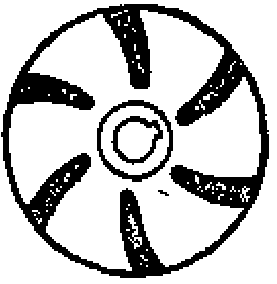
\includegraphics[width=3.5cm]{../pic/czjh1-ch4-34.png}
        \caption{}\label{fig:czjh1-4-34}
    \end{minipage}
    \qquad
    \begin{minipage}[b]{7cm}
        \centering
        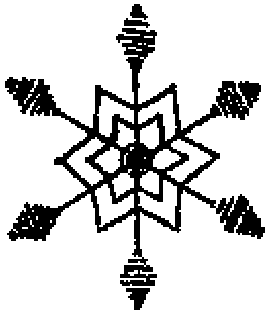
\includegraphics[width=3.5cm]{../pic/czjh1-ch4-35.png}
        \caption{}\label{fig:czjh1-4-35}
    \end{minipage}
\end{figure}

\begin{lianxi}

\xiaoti{举出几个中心对称图形的实例。}

\xiaoti{线段、射线、两条相交直线,是不是中心对称图形?如果是,指出对称中心的位置。}

\xiaoti{正三角形、五角星是不是中心对称图形?为什么?}

\end{lianxi}

